\documentclass[10pt]{article}
\usepackage[export]{adjustbox}
\usepackage{graphicx}
\begin{document}
	
	
\begin{tabbing}
	\hspace{1.75in}
	\huge{\bf Nagesh K} % Print the main header
\end{tabbing}
%------------------------------------------------
\hspace{-.05cm}\makebox[\linewidth]{\rule{20cm}{0.4pt}}
\vspace{.05 in} \\
\noindent\hspace{-1 in}
\begin{tabular}{@{}p{3.25in}p{3in}}
	
	No.214/1, 7\textsuperscript{th} Cross,             & {Phone:}  9739530539 \\
	Kurubarahalli, 
	& {E-mail:}  nagu1997@gmail.com\\
	Bangalore - 560086  
\end{tabular}

	\begin{figure}[h]
		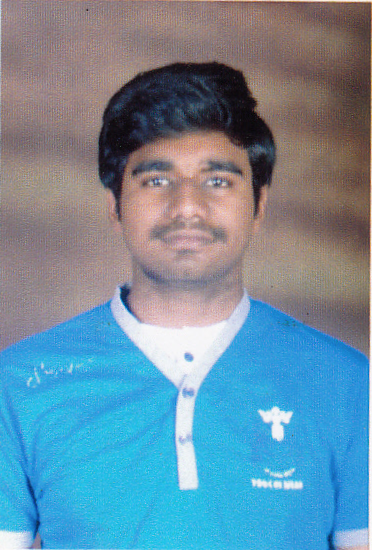
\includegraphics[width=0.2\textwidth,right]{photo.png}
	\end{figure}
	
	
		\underline{\textbf{\Large{Objective:}}}\\
		
		To constantly upgrade my knowledge and skills, help society through\\ innovations in technology and make a difference in whatever I do.\\
		
%	\hfill\\	
	\underline{\textbf{\Large{Education:}}}
	\vspace{-0.5cm}
	
	\hfill\\
	\hfill\\
	%\noindent\flushleft%\vspace{.3in}
	%\hspace{-0.9in}
	\begin{tabular}{|c|c|c|c|c|}
		\hline
		\bf Degree & \bf College/School & \bf University & \bf Passing Year & \bf  Percentage \\
		\hline
		Bachelor of & RV College of & VTU & 2019 & 9.03/10\\
		Engineering &  Engineering &  & (Pursuing) & (3 sems)\\
		\hline
		Pre-& S Nijalingappa & Karnataka & 2015 & 96\\
		University & PU College & Board & &\\
		\hline
		Secondary & Twinklers & Karnataka & 2013 & 96 \\
		School & High School & Board & & \\
		\hline
	\end{tabular}
	
	\vspace{0.5cm}	
	\underline{\textbf{\Large{List of Projects:}}}
	\begin{enumerate}
		\item{\underline{\textbf{\large{Robotic Arm:}}} This project aims at providing a remotely controlled substitute for the arm. This   also aims at industrial automation. This   project uses 5 servo motors to bring about various movements and ATMEGA 328 to control the servo motors.}
		\item{\underline{\textbf{\large{Trailblazer:}}} This project aims at developing a bot capable decoding realtime data. This uses the concept of line follower to follow the line while decoding the information on the ground. The information is in the form of black patches which is recognized using an IR sensor. Organized by NIT Surathkal.}
		\item{\underline{\textbf{\large{e-Yantra:}}} This project aims at tackling one of the basic challenges faced by the mars rover i.e. crossing the crater. This project uses concept of image processing to identify the obstacles, cavities etc. An efficient path is planned based on this information which is sent to the rover. Organized by IIT Bombay.}
		\item{\underline{\textbf{\large{LED Cube:}}} This project aims at developing a multipurpose cube for both education and entertainment purpose.It can be used as rubiks cube as well as an entertainment unit. It is 4X4X4 LED matrix replicating a Rubiks cube.}
		\item{\underline{\textbf{\large{Line Follower:}}} This project aims at developing a bot capable of following complex patterns. It can also be used  as a substitute for present rail system in industries. The prototype uses IR LEDs to recognize the white line.}
		\item{\underline{\textbf{\large{Snake Game:}}} This project aims at developing a game. It uses 64X64 graphical LCD for display. 8051 Microcontroller is used to interface the LCD and to accept the user inputs, based on which the snake is controlled.'}
	\end{enumerate}
	
	\hfill
	%\vspace{1cm}
	
		\underline{\textbf{\Large{Training and Internship:}}}
		\begin{itemize}
			\item{Conducted a 'Basic Robotics Workshop' for class 12 students.}
			\item{Attended a Workshop on "PCB Design".}\\
		\end{itemize}
		
		%\hfill 
		%\vspace{1cm}
		
		%\underline{\textbf{\Large{Research Publication:}}}
		%\begin{enumerate}
		%	Nil-
		%\end{enumerate}	
	
		\\
		
		\underline{\textbf{\Large{Technical Skills:}}}
		\begin{enumerate}
			\item{Programming languages C, Python and a basic understanding of \\embedded C}
			\item{Worked with ATmega 2560, 328 and 8051 Microcontrollers}
			\item {Basic Knowledge of signal analysis using MATLAB}
			\item{Mechanical skills like welding, drilling and worked with related tools and machines}
			\item{Analysis of electronic circuits and home wiring}
		\end{enumerate}
		
		\hfill 
		\hfill
	
			\underline{\textbf{\Large{Soft Skills:}}}
			\begin{itemize}
				\item{Hard working, dedicated and punctual}
				\item{Team work and responsibility}
				\item{leadership qualities}\\ 
			\end{itemize}
			\vspace{1cm}
			\hfill
			
		\underline{\textbf{\Large{Extra-Curricular Activities:}}}
		\begin{enumerate}
			\item{Volunteered as a student mentor at the 'The Akshay Patra Foundation', an NGO in Bangalore}
			\item {Active member of Rotract Club}
			\item{Been a 'Head Boy' in my school}	
		\end{enumerate}
		
		\hfill
		
			\underline{\textbf{\Large{Co-Curricular Activities:}}}
			\begin{itemize}
				\item{Part of "Astra', robotics club of RVCE}
				\item{Part of "CARV", acting club of RVCE}
				\item{Organized few inter-college competitions}
				\item{Participated in inter-college quiz contests}\\		
			\end{itemize}
			
			\underline{\textbf{\Large{Achievements:}}}
			\begin{enumerate}
				\item{Participated and won \textbf{1\textsuperscript{st}
					place in Engineer 2016,“Trailblazer”} event organized
					by NIT-Surathkal.}
				\item{Participated and won \textbf{4\textsuperscript{th}
					place in e-Yantra 2017,“Cross the Crater”} theme
					organized by IIT-Bombay.}
				
			\end{enumerate}
			
			
			\hfill
			
				\underline{\textbf{\Large{Personal details}}}
				
				\parbox{1.5\textwidth}{ % First block
					\begin{tabbing} % Enables tabbing
						\hspace{3cm} \= \hspace{4cm} \= \kill % Spacing within the block
						{ Father's Name} \> Keshava Kumar A\\
						{ Mother's Name} \> Asha P S\\
						{ Sex} \> Male\\
						{ Date of Birth} \> 23$^{rd}$ Jan 1998  \\ 
						{ Nationality} \> Indian \\
						{ Marital Status} \> Single
				\end{tabbing}}
				
				\hfill
				
				\underline{\textbf{\Large{Reference}}} 
				\begin{tabbing}
					\hspace{0.5cm}
					Dr. M Uttara Kumari\\
					\hspace{0.5cm}
					Professor, EC Department,\\
					\hspace{0.5cm}
					RV College of Engineering\\
					\hspace{0.5cm}
					{E-mail:}  nagu1997@gmail.com\\
					\hspace{0.5cm}
					Ph: 99453 36808\\
				\end{tabbing}
				
					\underline{\textbf{\Large{Declaration}}} \\
					
					I hereby declare that the above information is true to the best of my \\knowledge
					\\
					\hfill
					
					\underline{\textbf{\large{Date:}}}  {\em\today}
	
\end{document}